\documentclass[11pt,a4paper]{article}
\usepackage[utf8]{inputenc}
\usepackage[T1]{fontenc}
\usepackage[spanish,es-tabla]{babel}
\usepackage[margin=2.3cm]{geometry}
\usepackage{lmodern,microtype}
\usepackage{booktabs,graphicx,amsmath,array}
\usepackage[hidelinks]{hyperref}
\usepackage{caption}
\captionsetup{font=small,labelfont=bf}
\setlength{\parskip}{4pt}
\decimalcomma
\title{\textbf{Microsimulación de Pobreza}\\\large Un modelo de microsimulación macro-micro de pobreza y distribución del ingreso para el Perú\\\normalsize Nota metodológica y validación}
\author{Eric Torres Ramírez\\\small\texttt{etorresram@gmail.com}}
\date{Octubre de 2026}
\begin{document}
\maketitle
\vspace{-8pt}
\begin{abstract}
\noindent Esta nota documenta un modelo de microsimulación que combina los microdatos de la Encuesta Nacional de Hogares (ENAHO) del Perú con series macroeconómicas y del mercado laboral para proyectar la pobreza y la distribución del ingreso y construir escenarios contrafactuales. Sigue el enfoque de modelos de generación de ingresos del hogar (Bourguignon, Ferreira y Lustig, 2005) en su versión \emph{top-down} no paramétrica: un logit multinomial de estado laboral, uno de sector y ecuaciones de Mincer por segmento se estiman en la ENAHO 2019; la simulación reasigna estados laborales hasta cuadrar las metas agregadas, reescala los ingresos con el PBI sectorial, los precios y los agregados laborales, actualiza los ingresos no laborales y traslada el cambio del ingreso al gasto per cápita con el que el INEI mide la pobreza. Validado por \emph{backcasting} contra 2020--2024, el modelo reproduce la pobreza nacional con un error absoluto medio de @@EAM@@ puntos porcentuales. Acompañan a la nota el código reproducible (Python), una interfaz para usuarios no técnicos que corre el mismo motor en el navegador (JavaScript, con prueba de equivalencia) y un manual de usuario. Es una muestra de trabajo preparada para la consultoría del Grupo de Pobreza del BID \emph{Desarrollo de un modelo de micro-simulación}.
\end{abstract}

\section{Objetivo y alcance}
El modelo responde dos preguntas: (i) dada una trayectoria macroeconómica (PBI por sector, empleo, informalidad, inflación, transferencias, remesas), ¿qué pasa con la pobreza, la pobreza extrema y la desigualdad?; y (ii) ¿cuál es el impacto distributivo de un choque o de una política (un bono, un retiro extraordinario de fondos de pensiones, un cambio en Juntos o Pensión~65)? Está construido para un país, el Perú, pero el motor no contiene nada específico del país: opera sobre dos tablas (personas y hogares) con un diccionario de columnas fijo y sobre un diccionario de insumos macro, de modo que extenderlo a la base armonizada del BID exige solo reescribir el módulo de preparación de datos y la correspondencia sector--PBI.

\section{Datos}
\paragraph{Microdatos.} ENAHO anual 2019--2024 (INEI), módulos 200 (miembros), 300 (educación), 500 (empleo e ingresos) y Sumaria (ingresos, gastos y pobreza del hogar), descargados directamente del portal de microdatos del INEI con el script \texttt{00\_descargar.py}. El año base es 2019 (34\,565 hogares, 121\,007 personas, @@N14@@ de 14 años y más); 2020--2024 se usan solo para construir los insumos observados y para la validación. La base reproduce exactamente la pobreza oficial de cada año (20,2; 30,1; 25,9; 27,5; 29,0 y 27,6\,\%).

\paragraph{Ingreso laboral individual.} Suma de los nueve componentes del módulo 500 (ingreso principal y secundario, dependiente e independiente, monetario y en especie, extraordinarios), anualizados e imputados por el INEI, expresados por mes. Agregados por hogar, su correlación con el ingreso laboral de la Sumaria es 0,99.

\paragraph{Ingreso no laboral del hogar.} Nueve componentes de la Sumaria: Juntos, Pensión~65, otras transferencias públicas (Beca~18, bono gas, bonos extraordinarios, donaciones públicas), pensiones y transferencias privadas internas, remesas del exterior, rentas de la propiedad, alquiler imputado, ingresos extraordinarios y un residuo que cierra la cuenta con el ingreso neto total.

\paragraph{Estados laborales.} Para las personas de 14 años y más: inactivo, desocupado, ocupado informal y ocupado formal, según \texttt{ocu500} y \texttt{ocupinf} del INEI. El INEI no incluyó \texttt{ocupinf} en la base pública de 2024; la formalidad de ese año se imputa persona a persona con una regresión logística entrenada en 2023 sobre las variables que definen la informalidad oficial (categoría ocupacional, registro en SUNAT, tipo de contrato, tamaño de la empresa, afiliación a pensiones, sector, educación, edad y área), con un acierto de @@ACC_INFORM@@\,\% en una muestra de validación; la informalidad imputada de 2024 es @@INF24@@\,\%.

\paragraph{Sectores.} Seis ramas de la ocupación principal (CIIU Rev.~4): agropecuario y pesca; minería e hidrocarburos; manufactura; construcción; comercio; servicios (incluye electricidad y agua). Cada una tiene su serie de PBI real en BCRPData.

\paragraph{Series macro.} Descargadas por la API de BCRPData (\texttt{02\_macro.py}): PBI real por sector (millones de soles de 2007), IPC de Lima (promedio anual), remesas del exterior (millones de US\$) y tipo de cambio. Las líneas de pobreza por dominio y área, y las tasas de ocupación, desempleo e informalidad, se calculan de la ENAHO de cada año; en operación vendrían de la EPEN o de proyecciones. El cuadro~\ref{tab:ins} resume los insumos observados.

\begin{table}[h]\centering\footnotesize
\caption{Insumos observados usados en el \emph{backcasting} (variación acumulada respecto de 2019, \%, salvo niveles)}\label{tab:ins}
\begin{tabular}{lrrrrrrr}\toprule
Año & PBI real & IPC & Línea de & Ocupación & Informalidad & Ingreso laboral & Remesas \\
 & & & pobreza & (nivel) & (nivel) & real por ocupado & (S/) \\\midrule
@@TAB_INS@@
\bottomrule\end{tabular}
\par\smallskip\raggedright\footnotesize Fuente: BCRPData e INEI (ENAHO). Base 2019: tasa de ocupación @@OCUP0@@\,\%, desempleo @@DES0@@\,\%, informalidad @@INF0@@\,\%.
\end{table}

\section{Modelo base}
\paragraph{Elección ocupacional.} Logit multinomial de los cuatro estados sobre edad y su cuadrado, sexo, educación (cuatro niveles), jefatura, cónyuge, asistencia escolar, área, dominio geográfico, número de menores y de adultos en el hogar y la interacción sexo~$\times$~menores. Acierto en muestra @@ACC_ESTADO@@\,\%, pseudo-$R^2$ @@R2_ESTADO@@. De las probabilidades predichas se derivan $P(\text{ocupado})$, $P(\text{desocupado}\mid\text{no ocupado})$ y $P(\text{formal}\mid\text{ocupado})$, que ordenan quién cambia de estado cuando cambian los agregados.

\paragraph{Sector.} Logit multinomial de los seis sectores entre los ocupados, con las mismas covariables más la formalidad (acierto @@ACC_SECTOR@@\,\%, pseudo-$R^2$ @@R2_SECTOR@@). Para los no ocupados se predice con la formalidad más probable; el sector modal es el \emph{sector potencial}.

\paragraph{Ecuaciones de ingreso.} Mínimos cuadrados ponderados del logaritmo del ingreso laboral mensual por segmento: informal ($n=$ @@N_INF@@, $R^2=$ @@R2_INF@@, $\sigma=$ @@SIG_INF@@) y formal ($n=$ @@N_FOR@@, $R^2=$ @@R2_FOR@@, $\sigma=$ @@SIG_FOR@@), con las covariables anteriores y efectos de sector. Las brechas estimadas son las esperadas: la de las mujeres es @@MUJER_INF@@ en el segmento informal y @@MUJER_FOR@@ en el formal; el premio por educación universitaria es @@EDUC4_INF@@ y @@EDUC4_FOR@@. Cada persona conserva su residuo; a quien no está en un segmento se le asigna un residuo sorteado de la distribución empírica de ese segmento (semilla fija), de modo que los \emph{ingresos potenciales} formal e informal existen para todos y la simulación es determinista.

\section{Módulo de simulación}
Dado un escenario, el motor ejecuta siete pasos; el código de Python (\texttt{microsim/simular.py}) y el de JavaScript (\texttt{gui/motor.js}) implementan exactamente los mismos y una prueba automática verifica que coinciden.
\begin{enumerate}\itemsep2pt
\item \textbf{Reponderación.} Los factores de los hogares se escalan con el crecimiento poblacional; en el \emph{backcasting} se calibran además por \emph{raking} a los márgenes de población por sexo, grupo de edad y área.
\item \textbf{Ocupación y desempleo.} Si la meta de ocupados supera a la base, entran los no ocupados con mayor $P(\text{ocupado})$ hasta cubrir la diferencia ponderada; si es menor, salen los ocupados con menor probabilidad. Entre los no ocupados, los de mayor $P(\text{desocupado})$ cubren la meta de desempleo.
\item \textbf{Formalidad.} Igual mecanismo con $P(\text{formal}\mid\text{ocupado})$ hasta la meta de informalidad.
\item \textbf{Sectores.} Los nuevos ocupados entran en su sector potencial; luego los sectores en déficit respecto de la estructura meta toman de los sectores en superávit a los trabajadores con mayor probabilidad predicha de pertenecer al sector de destino.
\item \textbf{Ingresos laborales.} Quien sigue en su segmento conserva su ingreso observado; quien entra o cambia de segmento recibe su ingreso potencial, ajustado por el efecto de sector si cambia de rama. Después, el ingreso de cada sector $s$ se multiplica por
\[
f_s=\underbrace{\frac{g_{\text{lab}}\,\big(\mathrm{VA}_s/L_s\big)^{\pi}}{\sum_k \omega_k\,\big(\mathrm{VA}_k/L_k\big)^{\pi}}}_{\text{real}}\times\;\mathrm{IPC},
\]
donde $\mathrm{VA}_s$ es el PBI real del sector (factor respecto de la base), $L_s$ el empleo simulado del sector, $\omega_k$ la participación de cada sector en la masa salarial de 2019, $\pi$ el \emph{passthrough} del PBI sectorial por ocupado a los ingresos y $g_{\text{lab}}$ el crecimiento real del ingreso laboral medio (observado en la EPEN/ENAHO o fijado por el usuario). Sin $g_{\text{lab}}$ el modelo opera en modo ``solo PBI'' ($f_s=(\mathrm{VA}_s/L_s)^{\pi}\,\mathrm{IPC}$). Para el \emph{backcasting} se dispone además de factores observados por sector y por sector~$\times$~área.
\item \textbf{Ingresos no laborales y políticas.} Cada componente crece con su factor: Juntos, Pensión~65 y otras transferencias públicas con su ejecución; pensiones y transferencias privadas, alquiler imputado y residuo con la inflación; remesas con la serie del BCRP en soles; rentas con el PBI nominal. Dos instrumentos de política se modelan por fuera: un \emph{bono} (monto anual por hogar, deciles de gasto cubiertos y proporción consumida) y un \emph{retiro extraordinario de AFP} (proporción de afiliados que retira, identificados con la afiliación declarada en la ENAHO y un sorteo fijo; monto medio y proporción consumida).
\item \textbf{Gasto, líneas e indicadores.} La pobreza oficial del Perú se mide con el gasto; el modelo traslada el cambio del ingreso total del hogar al gasto per cápita, $g_t=g_0\,(Y_t/Y_0)^{\varepsilon}$, con $\varepsilon$ la elasticidad gasto--ingreso, y actualiza las líneas de pobreza total y extrema con su propia inflación (por dominio y área en el \emph{backcasting}). Se calculan incidencia, brecha y severidad de la pobreza, pobreza extrema, Gini del gasto y del ingreso, curvas de incidencia del crecimiento por decil, y desagregaciones por área, dominio y departamento.
\end{enumerate}
El escenario neutro (todos los factores en uno y las metas en sus valores de 2019) reproduce exactamente la pobreza oficial del año base, lo que verifica la consistencia interna del motor.

\section{Validación}
\paragraph{Backcasting.} Con el modelo estimado en 2019 y los insumos observados de cada año (cuadro~\ref{tab:ins}), más los bonos de la pandemia ingresados como política explícita (2020: S/\,1\,000 por hogar a los deciles 1--7; 2021: S/\,1\,225 a los deciles 1--4, aproximación de los bonos Universal Familiar, Rural, Independiente y Yanapay), el modelo reproduce la trayectoria de la pobreza 2020--2024 (cuadro~\ref{tab:bk}, figura~\ref{fig:bk}). El error absoluto medio nacional es de @@EAM@@ pp; el modelo capta el salto de la pandemia (@@POB2020@@\,\% simulado vs.\ 30,1\,\% oficial en 2020) y el nivel más alto de 2022--2024 pese al crecimiento del PBI, que en el modelo se explica por la caída del ingreso laboral real, el encarecimiento de la canasta por encima del IPC y la mayor informalidad. La pobreza urbana se subestima entre 2 y 4~pp y la rural se sobreestima entre 4 y 7~pp a partir de 2022: la curva de incidencia observada en el ámbito rural fue fuertemente favorable a los deciles medios (figura~\ref{fig:gic}), un patrón que un reescalado por sector no reproduce y que sugiere incorporar heterogeneidad regional del ingreso agropecuario en una versión completa.

\begin{table}[h]\centering\small
\caption{\emph{Backcasting} 2020--2024: pobreza oficial (INEI) y simulada (\% de la población)}\label{tab:bk}
\begin{tabular}{lrrrrrrrrr}\toprule
 & \multicolumn{3}{c}{Pobreza total} & \multicolumn{2}{c}{Pobreza extrema} & \multicolumn{2}{c}{Urbana} & \multicolumn{2}{c}{Rural}\\
\cmidrule(lr){2-4}\cmidrule(lr){5-6}\cmidrule(lr){7-8}\cmidrule(lr){9-10}
Año & Oficial & Simulada & Error (pp) & Oficial & Sim. & Oficial & Sim. & Oficial & Sim.\\\midrule
@@TAB_BK@@
\bottomrule\end{tabular}
\par\smallskip\raggedright\footnotesize Parámetros: ingresos laborales observados por sector y área, \emph{passthrough} 0,25, elasticidad gasto--ingreso 0,8, bonos de la pandemia explícitos.
\end{table}

\begin{figure}[h]\centering
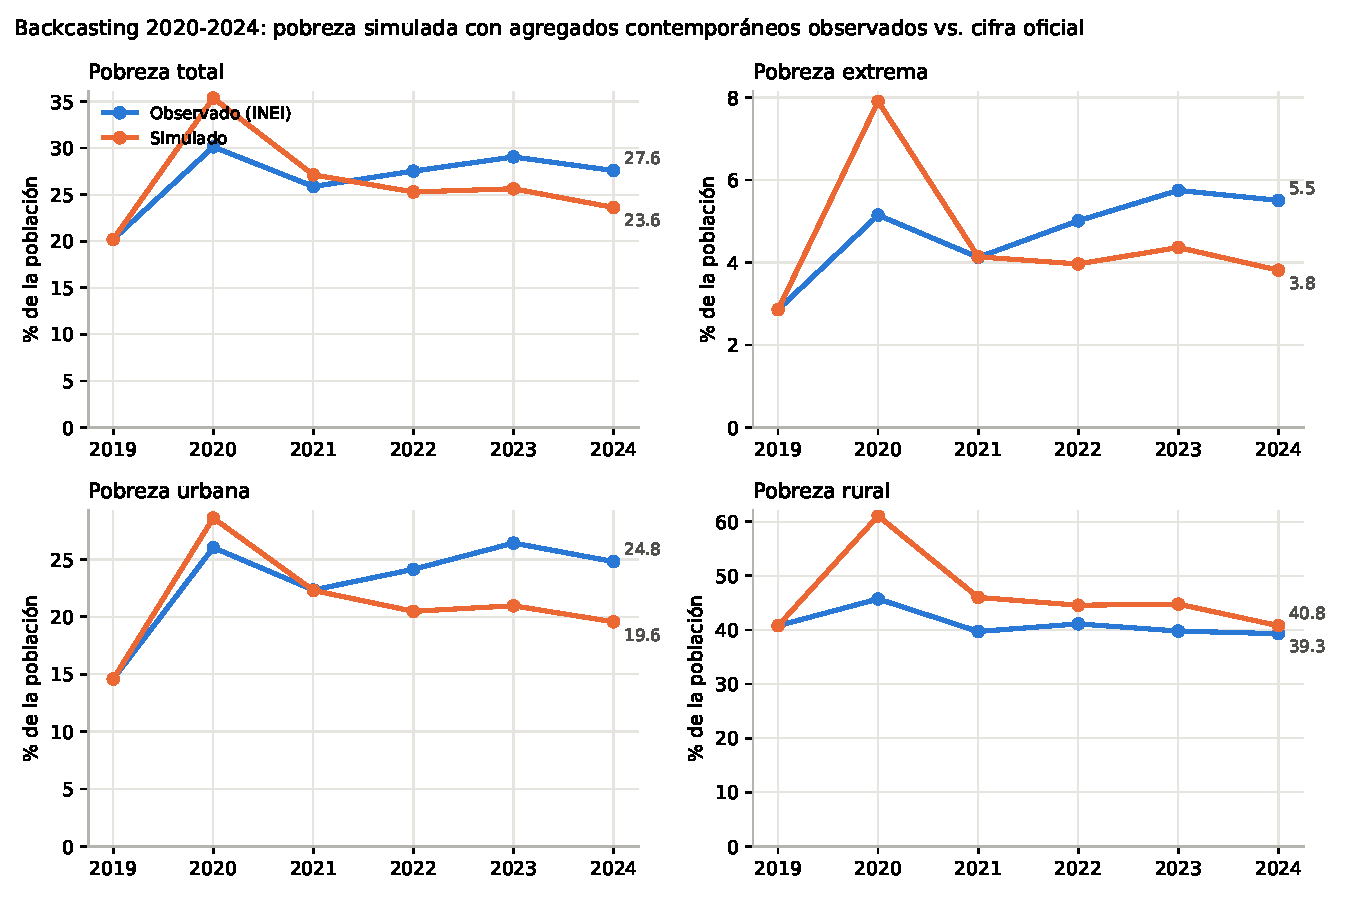
\includegraphics[width=\textwidth]{../output/figuras/backcast.pdf}
\caption{Pobreza simulada con insumos macro observados vs.\ cifra oficial, 2019--2024.}\label{fig:bk}
\end{figure}

\paragraph{Sensibilidad.} El cuadro~\ref{tab:sens} compara cuatro modos de traslado de la macroeconomía a los ingresos laborales y tres elasticidades. Dos lecciones. Primera, el PBI sectorial por ocupado \emph{no} es un buen predictor del ingreso laboral en el Perú de 2020--2024: el modo ``solo PBI'' sobreestima los ingresos y subestima la pobreza en @@SESGO_PBI@@~pp en promedio (con $\pi=1$), porque la participación del trabajo en el valor agregado cayó y la inflación erosionó los salarios reales; por eso el modelo exige, o bien un indicador observado del ingreso laboral medio (EPEN), o bien un supuesto explícito sobre su crecimiento real. Segunda, una elasticidad gasto--ingreso menor que uno (0,6--0,8) ajusta mejor que la transmisión completa, consistente con suavización del consumo; se adopta 0,8 como valor por defecto. Sin los bonos explícitos de la pandemia el error medio del modo adoptado sube a @@EAM_SIN_BONO@@~pp.

\begin{table}[h]\centering\small
\caption{Sensibilidad del \emph{backcasting}: error absoluto medio 2020--2024 (pp), \emph{passthrough} 0,25, bonos explícitos}\label{tab:sens}
\begin{tabular}{llrrrrr}\toprule
Modo de ingresos laborales & $\varepsilon$ & EAM & Sesgo & EAM extrema & EAM urbana & EAM rural\\\midrule
@@TAB_SENS@@
\bottomrule\end{tabular}
\end{table}

\begin{figure}[h]\centering
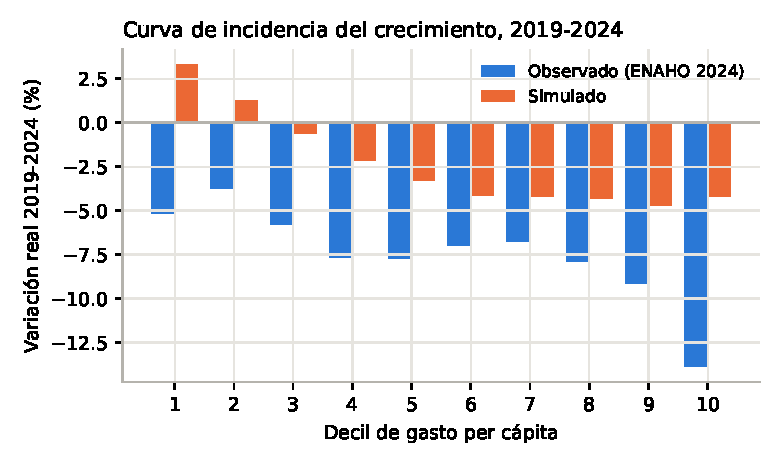
\includegraphics[width=0.55\textwidth]{../output/figuras/gic_2024.pdf}
\caption{Curva de incidencia del crecimiento 2019--2024, observada y simulada.}\label{fig:gic}
\end{figure}

\section{Interfaz, reproducibilidad y extensión}
\paragraph{Interfaz.} \texttt{gui/index.html} corre el motor en el navegador sobre la base exportada (91\,668 personas de 14+ y 34\,565 hogares, 12~MB sin comprimir, 2,7~MB comprimidos). El usuario carga un escenario predefinido (año base, cualquier año observado 2020--2024 con su cifra oficial al lado, un choque ilustrativo o el retiro de AFP), mueve controles agrupados (economía, mercado laboral, precios y líneas, ingresos no laborales, políticas, supuestos) y obtiene en alrededor de un segundo los indicadores, la curva de incidencia, la pobreza por dominio y por departamento y una tabla exportable como CSV; puede fijar un escenario como referencia para comparar dos. \texttt{07\_verificar\_gui.py} corre el mismo escenario en Python y en JavaScript y comprueba que los resultados coinciden (diferencias relativas menores que $10^{-3}$, atribuibles al orden de las sumas en punto flotante).

\paragraph{Reproducibilidad.} \texttt{run\_all.sh} ejecuta de principio a fin: descarga de la ENAHO del INEI, imputación de la informalidad 2024, preparación, series del BCRP, estimación, validación con figuras y tablas, exportación de la interfaz y prueba de equivalencia (unos diez minutos). El código es modular (paquete \texttt{microsim}: \texttt{config}, \texttt{preparar}, \texttt{estimar}, \texttt{simular}, \texttt{indicadores}, \texttt{macro}, \texttt{informalidad}), con semillas fijas y sin rutas absolutas. 

\paragraph{Qué haría la versión completa.} (i) Estimación por país sobre la base armonizada del BID con el mismo motor; (ii) reponderación demográfica con las proyecciones de población de CELADE; (iii) ingresos laborales por sector~$\times$~región alimentados con la EPEN o su equivalente en cada país; (iv) módulo de hogares para transferencias nuevas con reglas de elegibilidad (no solo deciles); (v) intervalos de incertidumbre por remuestreo de los residuos y de los parámetros; (vi) interfaz multi-país con los escenarios macro del Departamento de Investigación del Banco cargados por defecto.

\begin{thebibliography}{9}\small
\bibitem{bfl} Bourguignon, F., F.~H.~G.~Ferreira y N.~Lustig (eds.) (2005). \emph{The Microeconomics of Income Distribution Dynamics in East Asia and Latin America}. Banco Mundial y Oxford University Press.
\bibitem{olivieri} Olivieri, S., S.~Radyakin, S.~Kolenikov, M.~Lokshin, A.~Narayan y C.~Sánchez-Páramo (2014). \emph{Simulating Distributional Impacts of Macro-dynamics: Theory and Practical Applications}. Banco Mundial.
\bibitem{inei} INEI (2025). \emph{Perú: Evolución de la pobreza monetaria 2015--2024. Informe técnico}. Lima.
\bibitem{azuara} Azuara, O. y E.~Torres (2023). \emph{Labor Poverty in Latin America and the Caribbean}. BID.
\end{thebibliography}
\end{document}
